\chapter{Detecção de anomalias no painel}\label{cap_trabalho_academico}

Em alguns casos os dados podem apresentar registros que não parecem pertencer ao resto do conjunto, esses registros desviam muito do resto das observações e podem ser um problema na análise. Se o analista de dados conhecer o negócio, ele pode conseguir explicar a origem desses desvios. Por exemplo, imagine que uma loja registra um total de 10 vendas de produtos diariamente, e em uma determinada semana, sem explicação aparente, vendeu 1000 (diariamente também), após isso as vendas voltam para a casa dos 10 por dia. Claramente essa semana diferente deveria ser analisada para se entender as razões desse salto, mas se esse mesmo comportamento é registrado durante a \textit{black friday}, ele pode ser, justamente, o esperado para aquele período. O \textit{outlier}, como também são conhecidas essas anomalias, pode ter sido originada em algum \textit{bug} do sistema e isso precisa investigado com as outras áreas do negócio, além da TI.

Por causa dessas nuances a detecção de anomalias deve ser tratada com cuidado, porque analisando apenas os dados por si só não garante que os valores que se distanciam do normal são realmente anômalos. Na prática, é esperado que os dados sejam analisados apenas pelo analista, mas é importante que haja uma integração entre as diferentes áreas do negócio, no caso da JFRN, Varas e equipe de TI. 

\section{Distribuição dos dados}

A própria natureza do das Varas na Justiça já gera uma possível frequência maior de determinados Assuntos, então é esperado que uma Vara Penal receba uma alta demanda de Assuntos da competência dela, o mesmo raciocínio pode ser aplicado na 6ª Vara que é de Execução Fiscal. Mas, também existem Assuntos que aparecem na primeira distribuição dos Processos mas que não são da competência da Vara em que foi criado, e isso, apesar de não acontecer com uma frequência alta, acontece de forma pulverizada, então existem muitos Assuntos que possuem 1, 2 ou até 3 ocorrências, e poucos Assuntos que acontecem em frequências muito altas. Esse comportamento pode ser notado abaixo:
\pagebreak
\begin{figure}[h]
	\centering
	\subfloat[\centering Abril]{{		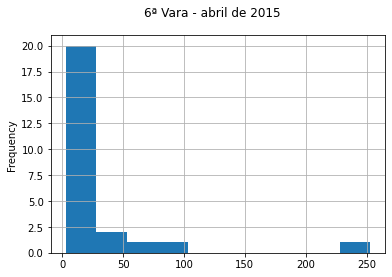
\includegraphics[scale=0.50]{./figures/analises/Vara_6_abril_2015.png} }}%
	\qquad
	\subfloat[\centering Setembro]{{		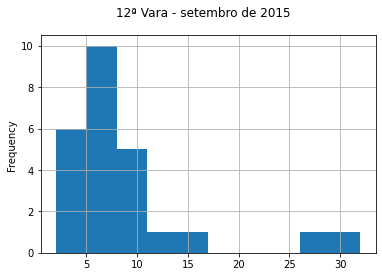
\includegraphics[scale=0.50]{./figures/analises/Vara_12_setembro_2015.png} }}%
	\caption{Comportamento da 6ª e 12ª Vara no ano de 2015}%
\end{figure}

\begin{figure}[h]
	\centering
	\subfloat[\centering Junho]{{		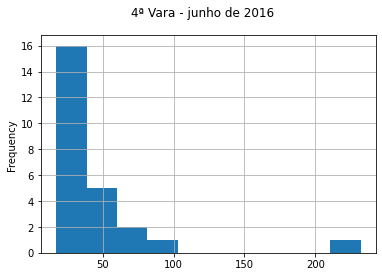
\includegraphics[scale=0.50]{./figures/analises/Vara_4_junho_2016.png} }}%
	\qquad
	\subfloat[\centering Janeiro]{{		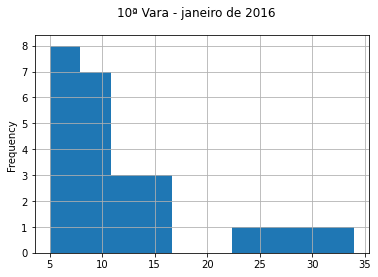
\includegraphics[scale=0.50]{./figures/analises/Vara_10_janeiro_2016.png} }}%
	\caption{Comportamento da 4ª e 10ª Vara no ano de 2016}%
\end{figure}

\begin{figure}[h]
	\centering
	\subfloat[\centering Setembro]{{		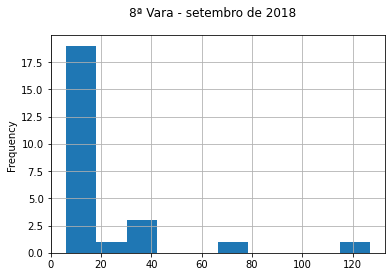
\includegraphics[scale=0.50]{./figures/analises/Vara_8_setembro_2018.png} }}%
	\qquad
	\subfloat[\centering Julho]{{		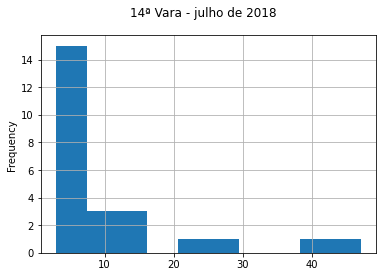
\includegraphics[scale=0.50]{./figures/analises/Vara_14_julho_2018.png} }}%
	\caption{Comportamento da 8ª e 14ª Vara no ano de 2018}%
\end{figure}
\pagebreak
No eixo horizontal são mostradas as frequências dos Assuntos, e no vertical a quantidade de Assuntos distintos, então essa concentração na esquerda indica que existem muitos processos com Assuntos diferentes mas em pequenas quantidades, e poucos (concentrados à direita) que possuem uma frequência alta, e são justamente esses, concentrados à direita, que pertencem à competência da Vara. Por isso que aparecem numa frequência tão superior aos outros, fazendo com que a distribuição desses processos não seja normal.

\section{Detecção de anomalias}

Como foi dito no início do capítulo, em alguns casos dados podem ser considerados diferentes demais para pertencerem a algum grupo e podem ser considerados \textit{outliers}, e em muitos casos isso leva em consideração a distribuição normal. 

\begin{figure}[h]
	\centering
	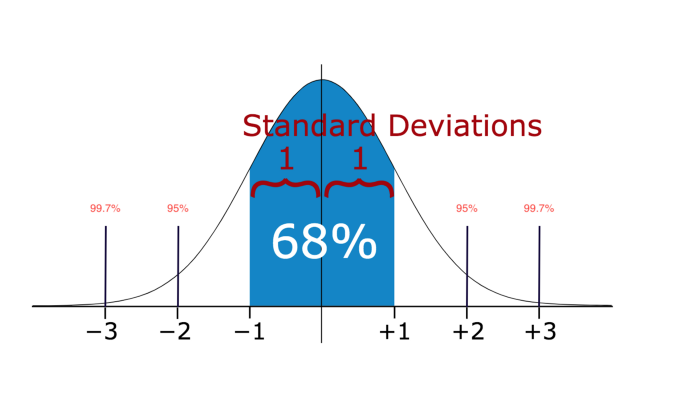
\includegraphics[scale=0.50]{./figures/cap3/dist_normal.png}
	\caption{Distribuição normal}
\end{figure}

Na distribuição normal 68\% dos dados estão dentro de 1 desvio padrão, representado pela letra grega sigma ($\sigma$), e 95\% estão dentro de 2, isso facilita a procura por \textit{outliers} porque a partir disso é possível determinar, de forma pragmática, o que pode ser um dado errado. Após isso, o analista de dados pode tentar entender melhor o que originou essa anomalia e decidir se isso é errado de fato ou se é um fenômeno genuíno, que possui uma explicação. No caso do painel, o objetivo não é tentar remover esses dados ou fazer qualquer operação neles, mas sim mostrar esses dados para o gestor e ele decide o que será feito. Nesse ponto se torna importante a integração entre a gestão das Varas e o time de TI, porque a partir disso as duas partes conseguem entender melhor os dados que estão sendo exibidos, os possíveis erros e as  causas dos \textit{outliers}, que nem sempre são resultados errados, longe disso, os \textit{outliers} aqui precisam ser mostrados para que sejam pesquisados e entendidos melhor.

A maioria das técnicas de detecção de \textit{outliers} se aplicam para dados com distribuição normal, e se os dados não forem normalizados, alguns passos são acrescidos, como a transformação logarítmica, para forçar a normalização. Esses métodos não atendem à função do painel porque a distribuição apresentada não é normal, e algumas características das Varas são perdidas se forçarmos a normalização.

%a média é pode ser fortemente influenciada pela existência de valores extremos num dataset, essa característica é importante porque as demandas variam de um ano para outro, já a mediana, que praticamente não sofre influência de outliers iria dividir o conjunto de dados na metade, não sendo muito útil porque é necessário mover a média de acordo com o período que é selecionado.
